%╔════════════════════════════╗
%║	  Szablon dostosował	  ║
%║	mgr inż. Dawid Kotlarski  ║
%║		  08.10.2022		  ║
%╚════════════════════════════╝
\documentclass[12pt,twoside,a4paper,openany]{article}

    % ------------------------------------------------------------------------
% PAKIETY
% ------------------------------------------------------------------------

%różne pakiety matematyczne, warto przejrzeć dokumentację, muszą być powyżej ustawień językowych.
\usepackage{mathrsfs}   %Różne symbole matematyczne opisane w katalogu ~\doc\latex\comprehensive. Zamienia \mathcal{L} ze zwykłego L na L-transformatę.
\usepackage{eucal}      %Różne symbole matematyczne.
\usepackage{amssymb}    %Różne symbole matematyczne.
\usepackage{amsmath}    %Dodatkowe funkcje matematyczne, np. polecenie \dfac{}{} skladajace ulamek w trybie wystawionym (porównaj $\dfrac{1}{2}$, a $\frac{1}{2}$).

%język polski i klawiatura
\usepackage[polish]{babel}
%\usepackage{qtimes} % czcionka Times new Roman
\usepackage[OT4]{polski}
%\usepackage[cp1250]{inputenc}                       %Strona kodowa polskich znaków.

%obsługa pdf'a
\usepackage[pdftex,usenames,dvipsnames]{color}      %Obsługa kolorów. Opcje usenames i dvipsnames wprowadzają dodatkowe nazwy kolorow.
\usepackage[pdftex,pagebackref=false,draft=false,pdfpagelabels=false,colorlinks=true,urlcolor=blue,linkcolor=black,citecolor=green,pdfstartview=FitH,pdfstartpage=1,pdfpagemode=UseOutlines,bookmarks=true,bookmarksopen=true,bookmarksopenlevel=2,bookmarksnumbered=true,pdfauthor={Dawid Kotlarski},pdftitle={Praca Inznierska},pdfsubject={},pdfkeywords={transient recovery voltage trv},unicode=true]{hyperref}   %Opcja pagebackref=true dotyczy bibliografii: pokazuje w spisie literatury numery stron, na których odwołano się do danej pozycji.

%bibliografia
%\usepackage[numbers,sort&compress]{natbib}  %Porządkuje zawartość odnośników do literatury, np. [2-4,6]. Musi być pod pdf'em, a styl bibliogfafii musi mieć nazwę z dodatkiem 'nat', np. \bibliographystyle{unsrtnat} (w kolejności cytowania).
\usepackage[
backend=biber,
style=numeric,
sorting=none
]{biblatex}
\addbibresource{bibliografia.bib}
\usepackage{hypernat}                       %Potrzebna pakietowi natbib do wspolpracy z pakietem hyperref (wazna kolejnosc: 1. hyperref, 2. natbib, 3. hypernat).

%grafika i geometria strony
\usepackage{extsizes}           %Dostepne inne rozmiary czcionek, np. 14 w poleceniu: \documentclass[14pt]{article}.
\usepackage[final]{graphicx}
\usepackage[a4paper,left=3.5cm,right=2.5cm,top=2.5cm,bottom=2.5cm]{geometry}

%strona tytułowa
\usepackage{strona_tytulowa}

%inne
\usepackage[hide]{todo}                     %Wprowadza polecenie \todo{treść}. Opcje pakietu: hide/show. Polecenie \todos ma byc na koncu dokumentu, wszystkie \todo{} po \todos sa ignorowane.
\usepackage[basic,physics]{circ}            %Wprowadza środowisko circuit do rysowania obwodów elektrycznych. Musi byc poniżej pakietow językowych.
\usepackage[sf,bf,outermarks]{titlesec}     %Troszczy się o wygląd tytułów rozdziałów (section, subsection, ...). sf oznacza czcionkę sans serif (typu arial), bf -- bold. U mnie: oddzielna linia dla naglowku paragraph. Patrz tez: tocloft -- lepiej robi format spisu tresci.
\usepackage{tocloft}                        %Troszczy się o format spisu trsci.
\usepackage{expdlist}    %Zmienia definicję środowiska description, daje większe możliwości wpływu na wygląd listy.
\usepackage{flafter}     %Wprowadza parametr [tb] do polecenia \suppressfloats[t] (polecenie to powoduje nie umieszczanie rysunkow, tabel itp. na stronach, na ktorych jest to polecenie (np. moze byc to stroma z tytulem rozdzialu, ktory chcemy zeby byl u samej gory, a nie np. pod rysunkiem)).
\usepackage{array}       %Ładniej drukuje tabelki (np. daje wiecej miejsca w komorkach -- nie są tak ścieśnione, jak bez tego pakietu).
\usepackage{listings}    %Listingi programow.
\usepackage[format=hang,labelsep=period,labelfont={bf,small},textfont=small]{caption}   %Formatuje podpisy pod rysunkami i tabelami. Parametr 'hang' powoduje wcięcie kolejnych linii podpisu na szerokosc nazwy podpisu, np. 'Rysunek 1.'.
\usepackage{appendix}    %Troszczy się o załączniki.
\usepackage{floatflt}    %Troszczy się o oblewanie rysunkow tekstem.
\usepackage{here}        %Wprowadza dodtkowy parametr umiejscowienia rysunków, tabel, itp.: H (duże). Umiejscawia obiekty ruchome dokladnie tam gdzie są w kodzie źródłowym dokumentu.
\usepackage{makeidx}     %Troszczy się o indeks (skorowidz).

%nieużywane, ale potencjalnie przydatne
\usepackage{sectsty}           %Formatuje nagłówki, np. żeby były kolorowe -- polecenie: \allsectionsfont{\color{Blue}}.
%\usepackage{version}           %Wersje dokumentu.

%============
\usepackage{longtable}			%tabelka
%============

%============
% Ustawienia listingów do kodu
%============

\usepackage{listings}
\usepackage{xcolor}

\definecolor{codegreen}{rgb}{0,0.6,0}
\definecolor{codegray}{rgb}{0.5,0.5,0.5}
\definecolor{codepurple}{rgb}{0.58,0,0.82}
\definecolor{backcolour}{rgb}{0.95,0.95,0.92}

% Definicja stylu "mystyle"
\lstdefinestyle{mystyle}{
	backgroundcolor=\color{backcolour},   
	commentstyle=\color{codegreen},
	keywordstyle=\color{blue},	%magenta
	numberstyle=\tiny\color{codegray},
	stringstyle=\color{codepurple},
	basicstyle=\ttfamily\footnotesize,
	breakatwhitespace=false,         
	breaklines=true,                 
	captionpos=b,                    
	keepspaces=true,                 
	numbers=left,                    
	numbersep=5pt,                  
	showspaces=false,                
	showstringspaces=false,
	showtabs=false,                  
	tabsize=2
}

\lstset{style=mystyle} % Deklaracja aktywnego stylu
%===========

%PAGINA GÓRNA I DOLNA
\usepackage{fancyhdr}          %Dodaje naglowki jakie się chce.
\pagestyle{fancy}
\fancyhf{}
% numery stron w paginie dolnej na srodku
\fancyfoot[C]{\scriptsize DOKUMENTACJA PROJEKTU - PROGRAMOWANIE URZĄDZEŃ MOBILNCH \\ 
\normalsize\sffamily  \thepage}


%\fancyhead[L]{\small\sffamily \nouppercase{\leftmark}}
\fancyhead[C]{\footnotesize \textit{AKADEMIA NAUK STOSOWANYCH W NOWYM SĄCZU}\\}

\renewcommand{\headrulewidth}{0.4pt}
\renewcommand{\footrulewidth}{0.4pt}

    % ------------------------------------------------------------------------
% USTAWIENIA
% ------------------------------------------------------------------------

% ------------------------------------------------------------------------
%   Kropki po numerach sekcji, podsekcji, itd.
%   Np. 1.2. Tytuł podrozdziału
% ------------------------------------------------------------------------
\makeatletter
    \def\numberline#1{\hb@xt@\@tempdima{#1.\hfil}}                      %kropki w spisie treści
    \renewcommand*\@seccntformat[1]{\csname the#1\endcsname.\enspace}   %kropki w treści dokumentu
\makeatother

% ------------------------------------------------------------------------
%   Numeracja równań, rysunków i tabel
%   Np.: (1.2), gdzie:
%   1 - numer sekcji, 2 - numer równania, rysunku, tabeli
%   Uwaga ogólna: o otoczeniu figure ma być najpierw \caption{}, potem \label{}, inaczej odnośnik nie działa!
% ------------------------------------------------------------------------
\makeatletter
    \@addtoreset{equation}{section} %resetuje licznik po rozpoczęciu nowej sekcji
    \renewcommand{\theequation}{{\thesection}.\@arabic\c@equation} %dodaje kropki

    \@addtoreset{figure}{section}
    \renewcommand{\thefigure}{{\thesection}.\@arabic\c@figure}

    \@addtoreset{table}{section}
    \renewcommand{\thetable}{{\thesection}.\@arabic\c@table}
\makeatother

% ------------------------------------------------------------------------
% Tablica
% ------------------------------------------------------------------------
\newenvironment{tabela}[3]
{
    \begin{table}[!htb]
    \centering
    \caption[#1]{#2}
    \vskip 9pt
    #3
}{
    \end{table}
}

% ------------------------------------------------------------------------
% Dostosowanie wyglądu pozycji listy \todos, np. zamiast 'p.' jest 'str.'
% ------------------------------------------------------------------------
\renewcommand{\todoitem}[2]{%
    \item \label{todo:\thetodo}%
    \ifx#1\todomark%
        \else\textbf{#1 }%
    \fi%
    (str.~\pageref{todopage:\thetodo})\ #2}
\renewcommand{\todoname}{Do zrobienia...}
\renewcommand{\todomark}{~uzupełnić}

% ------------------------------------------------------------------------
% Definicje
% ------------------------------------------------------------------------
\def\nonumsection#1{%
    \section*{#1}%
    \addcontentsline{toc}{section}{#1}%
    }
\def\nonumsubsection#1{%
    \subsection*{#1}%
    \addcontentsline{toc}{subsection}{#1}%
    }
\reversemarginpar %umieszcza notki po lewej stronie, czyli tam gdzie jest więcej miejsca
\def\notka#1{%
    \marginpar{\footnotesize{#1}}%
    }
\def\mathcal#1{%
    \mathscr{#1}%
    }
\newcommand{\atp}{ATP/EMTP} % Inaczej: \def\atp{ATP/EMTP}

% ------------------------------------------------------------------------
% Inne
% ------------------------------------------------------------------------
\frenchspacing                      
\hyphenation{ATP/-EMTP}             %dzielenie wyrazu w danym miejscu
\setlength{\parskip}{3pt}           %odstęp pomiędzy akapitami
\linespread{1.3}                    %odstęp pomiędzy liniami (interlinia)
\setcounter{tocdepth}{4}            %uwzględnianie w spisie treści czterech poziomów sekcji
\setcounter{secnumdepth}{4}         %numerowanie do czwartego poziomu sekcji 
\titleformat{\paragraph}[hang]      %wygląd nagłówków
{\normalfont\sffamily\bfseries}{\theparagraph}{1em}{}



    %polecenia zdefiniowane w pakiecie strona_tytulowa.sty
    \title{Runly: Running App}		%...Wpisać nazwę projektu...
    
    \authorI{Łukasz Skraba}
    \authorII{Bartosz Tobiasz}		%jeśli są dwie osoby w projekcie to zostawiamy:    \authorII{}
		
	\uczelnia{AKADEMIA NAUK STOSOWANYCH \\W NOWYM SĄCZU}
    \instytut{Wydział Nauk Inżynieryjnych}
    \kierunek{Katedra Informatyki}
    \praca{DOKUMENTACJA PROJEKTOWA}
    \przedmiot{PROGRAMOWANIE URZĄDZEŃ MOBILNYCH}
    \prowadzacy{mgr inż. Dawid Kotlarski}
    \rok{2022}


%definicja składni mikrotik
\usepackage{fancyvrb}
\DefineVerbatimEnvironment{MT}{Verbatim}%
{commandchars=\+\[\],fontsize=\small,formatcom=\color{red},frame=lines,baselinestretch=1,} 
\let\mt\verb 
%zakonczenie definicji składni mikrotik

\usepackage{fancyhdr}    %biblioteka do nagłówka i stopki

			
\begin{document}
   
    \renewcommand{\figurename}{Rys.}    %musi byc pod \begin{document}, bo w~tym miejscu pakiet 'babel' narzuca swoje ustawienia
    \renewcommand{\tablename}{Tab.}     %j.w.
    \thispagestyle{empty}               %na tej stronie: brak numeru
    \stronatytulowa                     %strona tytułowa tworzona przez pakiet strona_tytulowa.tex
 
 \pagestyle{fancy}

    \newpage

    %formatowanie spisu treści i~nagłówków
    \renewcommand{\cftbeforesecskip}{8pt}
    \renewcommand{\cftsecafterpnum}{\vskip 8pt}
    \renewcommand{\cftparskip}{3pt}
    \renewcommand{\cfttoctitlefont}{\Large\bfseries\sffamily}
    \renewcommand{\cftsecfont}{\bfseries\sffamily}
    \renewcommand{\cftsubsecfont}{\sffamily}
    \renewcommand{\cftsubsubsecfont}{\sffamily}
    \renewcommand{\cftparafont}{\sffamily}
    %koniec formatowania spisu treści i nagłówków
     
    \tableofcontents    %spis treści
    \thispagestyle{fancy}
    \newpage

    
    \newpage

    
%%%%%%%%%%%%%%%%%%% treść główna dokumentu %%%%%%%%%%%%%%%%%%%%%%%%%

   	\newpage
\section{Ogólne określenie wymagań}		%1
%Ogólne określenie wymagań i zakresu programu (Czyli zleceniodawca określa wymagania programu) 




\subsection{Opis działania}  %1.1       

\hspace{0.60cm}Aplikacja na urządzenia mobilne umożliwiająca monitoring dokonań sportowych w dziedzinie biegania. Program ma umożliwić monitorowanie naszej aktywności biegowej. Aplikacja ma zapisywać przede wszystkim czas treningu, dystans, trasę uzyskaną dzięki modułowi GPS oraz intensywność treningu (np. wyliczając średnie tempo, średnią i maksymalną prędkość oraz skalone kalorie). Kożystając z aplikacji mamy mieć możliwość szczegółowej weryfikacji danych treningu, zarówno w trakcie jego trwania jak i po jego zakończeniu. Dodatkowo w podsumowaniu dzięki współpracy programu z GPS-em, można także spawdzić informacje o najniższym i najwyższym punkcie trasy. Szczegółowe statystyki mają pozwolić na analizę postępów i wyciągnięcie wniosków na przyszłość.

\hspace{0.60cm}Treningi mają być zapisywane w pamięci. Użytkownik ma mieć możliwość zobaczenia statystyk wybranego treningu.

\hspace{0.60cm}Aplikacja ma za zadanie także motywować nas do ćwiczeń, np. wysyłając nam powiadomienia, w ustalonym przez użytkownika momencie, o tym, że nie odbyliśmy jeszcze treningu.

\hspace{0.60cm}Poza pomiarami w trakcie treningu, aplikacja ma także liczyć kroki, kiedy działa w tle.






\subsection{Opis wyglądu}  %1.2


\hspace{0.60cm}Na głównej stronie treningu, którą widzi użytkownik po otwarciu aplikacji, Powinny znajdować się takie informacje jak:
\begin{itemize}
	
	\item czas trwania aktywności,
	\item prędkość w danym momencie, 
	\item średnia prędkość,
	\item dystans, 
	\item spalone kalorie, 
\end{itemize}

\hspace{0.60cm}Oprócz tego na stronie treningu Rys. \ref{rys:rysunek001} (s. \pageref{rys:rysunek001}) powinna znajdować się mapa, na której będzie pokazana aktualna pozycja uzytkownika, oraz przebyta trasa.

\hspace{0.60cm}Po zakończonym treningu aplikacja ma pokazać całą przebytą trasę na mapie oraz dać dostęp do szczegółowych statystyk treningu Rys. \ref{rys:rysunek002} (s. \pageref{rys:rysunek002}). Użytkownik ma mieć podgląd na wszystkie możliwe dane.

\begin{figure}[!htb]
	\centering
	\begin{minipage}{.5\textwidth}
		\centering
		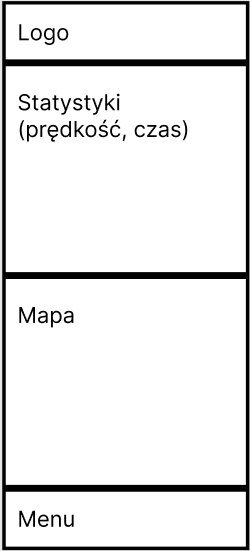
\includegraphics[width=.4\linewidth]{rys/ekran_treningu.png}
		\caption{Ekran treningu}
		\label{rys:rysunek001}
	\end{minipage}%
	\begin{minipage}{.5\textwidth}
		\centering
		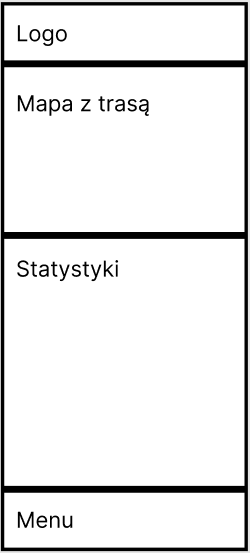
\includegraphics[width=.4\linewidth]{rys/ekran_podsumowania.png}
		\caption{Ekran podsumowania}
		\label{rys:rysunek002}
	\end{minipage}
\end{figure}

\hspace{0.60cm}Ekran krokomierza Rys. \ref{rys:rysunek003} (s. \pageref{rys:rysunek003}) ma zawierać tylko liczbę zrobionych w biezacym dniu kroków.

\begin{figure}[!htb]
	\centering
	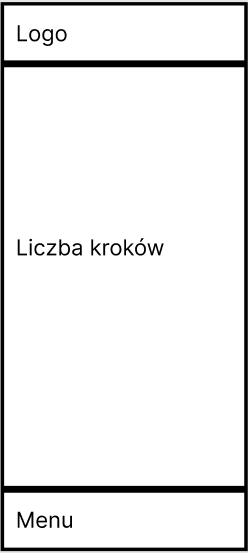
\includegraphics[width=.2\linewidth]{rys/ekran_krokomierza.png}
	\caption{Ekran krokomierza}
	\label{rys:rysunek003}
\end{figure}


\hspace{0.60cm}Na dole aplikacji ma się znajdować menu za pomocą którego użytkownik może się przełączać pomiędzy ekranem krokomierza, treningu, odbytymi treningami i ustawieniami.

\hspace{0.60cm}Ekran zawierający historię odbytych treningów powinien przedstawiać je w postaci list. Ustawienia też powinny być przedstawione w postaci listy. 
 
   \newpage
\section{Określenie wymagań szczegółowych}		%2


\hspace{0.60cm}Aplikacja zostanie napisana korzystając z Xamarin.Forms. Jest to środowisko umożliwiające tworzenie aplikacji za pomocą języka XAML oraz kodu w języku C\#.

\hspace{0.60cm}Aplikacja będzie podzielona na podstrony. Na dole będzie znajdować się menu z opcjami. Wybór poszczególnej opcji w menu wyświetli daną podstronę w ekranie aplikacji.




   	\newpage
\section{Projektowanie}		%3
%Opis przygotowania narzędzi (git, visual studio). Wybór i opis bibliotek, klas. Szkic layoutów. Pseudo kody. Opisy wykorzystanych algorytmów (np. algorytm sortowania). Dokładniejsze określenie założeń i działania aplikacji, (np.: ten przycisk otworzy takie okno a w tym oknie wpisujemy takie dane).




   	\newpage
\section{Implementacja}		%4
%Wkleić szkielet kodu, wraz z komentarzami. Opisać zmienne, struktury do czego służą. Opisać procedury, metody co wykonują. Opisać nowe zdefiniowane klasy. Opisać dziedziczenie. Opisać nowo utworzone pliki za co odpowiadają.




   	\newpage
\section{Testowanie}	%5
%Opisujemy testy, sprawdzamy czy nie generuje błędów.



   	\newpage
\section{Podręcznik użytkownika}  %6
%Opis jak używać programu. Mogą być z zrzut ekranu razem z opisem. 



       
%%%%%%%%%%%%%%%%%%% koniec treść główna dokumentu %%%%%%%%%%%%%%%%%%%%%
	\newpage
    \addcontentsline{toc}{section}{Literatura}  
	\printbibliography

    \newpage
    \hypersetup{linkcolor=black}
    \renewcommand{\cftparskip}{3pt}
    \clearpage
    \renewcommand{\cftloftitlefont}{\Large\bfseries\sffamily}
    \listoffigures
    \addcontentsline{toc}{section}{Spis rysunków}
	\thispagestyle{fancy}
	
    \newpage
    \renewcommand{\cftlottitlefont}{\Large\bfseries\sffamily}
    \def\listtablename{Spis tabel}
    \addcontentsline{toc}{section}{Spis tabel}\listoftables 
	\thispagestyle{fancy}
	
	\newpage
	\renewcommand{\cftlottitlefont}{\Large\bfseries\sffamily}
	\renewcommand\lstlistlistingname{Spis listingów}
	\addcontentsline{toc}{section}{Spis listingów}\lstlistoflistings 
	\thispagestyle{fancy}
	


    %lista rzeczy do zrobienia: wypisuje na koñcu dokumentu, patrz: pakiet todo.sty
    \todos
    %koniec listy rzeczy do zrobienia
\end{document}
